\documentclass[12pt,a4paper]{../krautsourcing/homework}
\usepackage[utf8]{inputenc}
\usepackage[ngerman]{babel}
\usepackage[T1]{fontenc}
\usepackage{amsmath}
\usepackage{graphicx}
\usepackage{amsfonts}
\usepackage{amssymb}
\usepackage{lmodern}
\usepackage{amsmath}
\usepackage{amssymb}
\usepackage{paralist}
\usepackage{tabularx}
\usepackage{tikz}
\usetikzlibrary{automata,positioning,petri,calc}

\author{Ruben Felgenhauer,\\Alexander Hildebrandt,\\Leonhard Reichenbach}
\datef{22}{11}{2015}
%\date{\today}
\course{Formale Grundlagen der Informatik II}
\sheet{6}
\sectionprefix{Übungsaufgabe \thesheet.}
\subsectionprefix{\thesheet.}
\subsubsectioncounter{\alph{subsubsection}}
\group{06}
\subsubsectionprefix{(}
\subsubsectionsuffix{)}

\begin{document}

\makeheadline

\addtocounter{section}{2}

\section{}
%%
\subsection{}

\newcommand{\VC}{\text{VC}}
\newcommand{\LT}{\text{LT}}
%\newcommand{\mcol}[1][c]{>{\(}#1<{\)}}
\newcommand{\vor}{\mathrel{\textbf{vor}}}

\renewcommand{\arraystretch}{1.2}

\centerline{\begin{tabular}{|>{\(}c<{\)}|>{\(}c<{\)}|>{\(}c<{\)}|>{\(}c<{\)}|
                 >{\(}c<{\)}|>{\(}c<{\)}|>{\(}c<{\)}|>{\(}c<{\)}|}
\hline
\multicolumn{2}{|c|}{\(p_0\)} & \multicolumn{2}{c|}{\(p_1\)} & \multicolumn{2}{c|}{\(p_2\)} & \multicolumn{2}{c|}{\(p_3\)}
\\ \hline
i & VC(\phi_{i}) & i & VC(\phi_{i}) & i & VC(\phi_{i}) & i & VC(\phi_{i})
\\ \hline
01 & (1,0,0,0) & 11 & (1,1,0,0) & 21 & (0,0,1,0) & 31 & (0,0,0,1) \\
02 & (2,0,0,0) & 12 & (1,2,0,2) & 22 & (2,0,2,0) & 32 & (0,0,1,2) \\
03 & (3,3,0,1) & 13 & (1,3,0,1) & 23 & (2,0,3,4) & 33 & (0,0,1,3) \\
04 & (4,3,1,3) & 14 & (1,4,0,1) & 24 & (2,4,4,4) & 34 & (0,0,1,4) \\
05 & (5,3,1,3) & 15 & (2,5,5,4) & 25 & (2,4,5,4) & 35 & (5,3,1,5) \\
06 & (6,3,1,3) & 16 & (5,6,5,6) & 26 & (6,4,6,4) & 36 & (5,3,1,6) \\
\hline
\end{tabular}}

\subsection{}

Wir wählen die vier Ereignisse \(\phi_{03}\), \(\phi_{12}\), \(\phi_{26}\) und \(\phi_{31}\), denn es gilt: \\
\(\begin{aligned}
\phi_{31} \vor \phi_{12} \vor \phi_{03} \vor \phi_{26} \
& \Leftrightarrow 
\VC(\phi_{31}) < \VC(\phi_{12}) < \VC(\phi_{03}) < \VC(\phi_{26})                                                                                                                                                                                                                                                                                                                                               
\\
& \Leftrightarrow 
(0,0,0,1) < (1,2,0,2) < (3,3,0,1) < (6,4,6,4)
\end{aligned}\)
\\
Aufgrund der Transitivität der Relation gilt, dass alle Ereignisse paarweise zueinander durch \(\vor\) angeordnet sind.

\subsection{}
Wir wählen die vier Ereignisse \(\phi_{02}\) mit \(\VC(\phi_{02}) = (2,0,0,0)\), \(\phi_{11}\) mit \(\VC(\phi_{11}) = (1,1,0,0)\), \(\phi_{21}\) mit \(\VC(\phi_{21}) = (0,0,1,0)\) und \(\phi_{31}\) mit \(\VC(\phi_{31}) = (0,0,0,1)\), da all diese Ereignisse paarweise zueinander unabhängig sind.

\subsection{}

\centerline{\begin{tabular}{|>{\(}c<{\)}|>{\(}c<{\)}|>{\(}c<{\)}|>{\(}c<{\)}|
                 >{\(}c<{\)}|>{\(}c<{\)}|>{\(}c<{\)}|>{\(}c<{\)}|}
\hline
\multicolumn{2}{|c|}{\(p_0\)} & \multicolumn{2}{c|}{\(p_1\)} & \multicolumn{2}{c|}{\(p_2\)} & \multicolumn{2}{c|}{\(p_3\)} \\ \hline
i & (\LT(\phi_{i}),p_i) & i & (\LT(\phi_{i}),p_i) & i & (\LT(\phi_{i}),p_i) & i & (\LT(\phi_{i}),p_i) 
\\ \hline
01 & (1,0) & 11 & (2,1) & 21 & (1,2) & 31 & (1,3) \\
02 & (2,0) & 12 & (3,1) & 22 & (3,2) & 32 & (2,3) \\
03 & (5,0) & 13 & (4,1) & 23 & (5,2) & 33 & (3,3) \\
\hline
\end{tabular}}
\vspace{2mm}
\(
\phi_{01} \vor \phi_{21} \vor \phi_{31} \vor \phi_{02} \vor \phi_{11} \vor \phi_{32} \vor \phi_{12} \vor \phi_{22} \vor \phi_{33} \vor \phi_{13} \vor \phi_{03} \vor \phi_{23}
\)
\subsection{}
\centerline{
\begin{tikzpicture}[auto, baseline, node distance=10mm, kot/.style={place,draw}]
\node[kot]             (01) {\(\phi_{01}\)};
\node[kot,below=of 01] (11) {\(\phi_{11}\)};
\node[kot,below=of 11] (21) {\(\phi_{21}\)};
\node[kot,below=of 21] (31) {\(\phi_{31}\)};
%
\node[kot,right=of 11] (12) {\(\phi_{12}\)};
\node[kot,right=of 12|-01] (02) {\(\phi_{02}\)};
\node[kot,right=of 12|-21] (22) {\(\phi_{22}\)};
\node[kot,right=of 12|-31] (32) {\(\phi_{32}\)};
%
\node[kot,right=of 02|-02] (03) {\(\phi_{03}\)};
\node[kot,right=of 02|-12] (13) {\(\phi_{13}\)};
\node[kot,right=of 02|-22] (23) {\(\phi_{23}\)};
\node[kot,right=of 02|-32] (33) {\(\phi_{33}\)};
%
\node[kot,right=of 03] (04) {\(\phi_{04}\)};
\node[kot,right=of 13] (14) {\(\phi_{14}\)};
\node[kot,right=of 23] (24) {\(\phi_{24}\)};
\node[kot,right=of 33] (34) {\(\phi_{34}\)};
%
\node[kot,right=of 04]     (05) {\(\phi_{05}\)};
\node[kot,right=of 05|-14] (15) {\(\phi_{15}\)};
\node[kot,right=of 05|-24] (25) {\(\phi_{25}\)};
\node[kot,right=of 34]     (35) {\(\phi_{35}\)};
%
\node[kot,right=of 15|-05] (06) {\(\phi_{06}\)};
\node[kot,right=of 15|-25] (26) {\(\phi_{26}\)};
\node[kot,right=of 26|-15] (16) {\(\phi_{16}\)};
\node[kot,right=of 26|-35] (36) {\(\phi_{36}\)};
%
\path[->]
	(01) edge (02) 
	(02) edge (03)
	(03) edge (04)
	(04) edge (05)
	(05) edge (06)
%
	(01) edge (11)
	(02) edge (22)
	(05) edge (35)
	(06) edge (26)
%
	(11) edge (12) 
	(12) edge (13)
	(13) edge (14)
	(14) edge (15)
	(15) edge (16)
%
	(13) edge (03)
	(14) edge (24)
%
	(21) edge (22) 
	(22) edge (23)
	(23) edge (24)
	(24) edge (25)
	(25) edge (26)
%	
	(21) edge (32)
	(25) edge (15)
%
	(31) edge (32) 
	(32) edge (33)
	(33) edge (34)
	(34) edge (35)
	(35) edge (36)
%	
	(31) edge (12)
	(33) edge (04)
	(34) edge (23)
	(36) edge (16)
; %-draw-%
\end{tikzpicture}
}

\vspace{10mm}
\subsection{}
\newcommand{\dummy}[1]{#1}
\renewcommand{\dummy}[1]{}


\centerline{\scalebox{0.9}{
\begin{tikzpicture}[auto, baseline, node distance=15mm]
\node[place] (01) {\dummy{01}};
\node[place,below=of 01] (11) {\dummy{11}};
\node[place,below=of 11] (21) {\dummy{21}};
\node[place,below=of 21] (31) {\dummy{31}};
%
\node[place,right=of 11] (12) {\dummy{12}};
\node[place,right=of 12|-01] (02) {\dummy{02}};
\node[place,right=of 12|-21] (22) {\dummy{22}};
\node[place,right=of 12|-31] (32) {\dummy{32}};
%
\node[place,right=of 02|-02] (03) {\dummy{03}};
\node[place,right=of 02|-12] (13) {\dummy{13}};
\node[place,right=of 02|-22] (23) {\dummy{23}};
\node[place,right=of 02|-32] (33) {\dummy{33}};
%
\node[place,right=of 03] (04) {\dummy{04}};
\node[place,right=of 13] (14) {\dummy{14}};
\node[place,right=of 23] (24) {\dummy{24}};
\node[place,right=of 33] (34) {\dummy{34}};
%
\node[place,right=of 04]     (05) {\dummy{05}};
\node[place,right=of 05|-14] (15) {\dummy{15}};
\node[place,right=of 05|-24] (25) {\dummy{25}};
\node[place,right=of 34]     (35) {\dummy{35}};
%
\node[place,right=of 15|-05] (06) {\dummy{06}};
\node[place,right=of 15|-25] (26) {\dummy{26}};
\node[place,right=of 26|-15] (16) {\dummy{16}};
\node[place,right=of 26|-35] (36) {\dummy{36}};
%
\node[transition,at=($(01)!0.5!(02)$)] (01-02) {\dummy{01-02}};
\node[transition,at=($(02)!0.5!(03)$)] (02-03) {\dummy{02-03}};
\node[transition,at=($(03)!0.5!(04)$)] (03-04) {\dummy{03-04}};
\node[transition,at=($(04)!0.5!(05)$)] (04-05) {\dummy{04-05}};
\node[transition,at=($(05)!0.5!(06)$)] (05-06) {\dummy{05-06}};
\node[transition,at=($(01)!0.5!(11)$)] (01-11) {\dummy{01-11}};
%\node[transition,at=($(02)!0.5!(22)$)] (02-22) {\dummy{02-22}};
\node[transition,at=($(02)!0.3!(22)$)] (02-22) {\dummy{02-22}};
\node[transition,at=($(05)!0.5!(35)$)] (05-35) {\dummy{05-35}};
%\node[transition,at=($(06)!0.5!(26)$)] (06-26) {\dummy{06-26}};
\node[transition,at=($(06)!0.3!(26)$)] (06-26) {\dummy{06-26}};
\node[transition,at=($(11)!0.5!(12)$)] (11-12) {\dummy{11-12}};
%\node[transition,at=($(12)!0.5!(13)$)] (12-13) {\dummy{12-13}};
\node[transition,at=($(12)!0.3!(13)$)] (12-13) {\dummy{12-13}};
\node[transition,at=($(13)!0.5!(14)$)] (13-14) {\dummy{13-14}};
\node[transition,at=($(14)!0.3!(15)$)] (14-15) {\dummy{14-15}};
%\node[transition,at=($(14)!0.5!(15)$)] (14-15) {\dummy{14-15}};
%\node[transition,at=($(15)!0.5!(16)$)] (15-16) {\dummy{15-16}};
\node[transition,at=($(15)!0.3!(16)$)] (15-16) {\dummy{15-16}};
\node[transition,at=($(13)!0.5!(03)$)] (13-03) {\dummy{13-03}};
\node[transition,at=($(14)!0.5!(24)$)] (14-24) {\dummy{14-24}};
\node[transition,at=($(21)!0.5!(22)$)] (21-22) {\dummy{21-22}};
\node[transition,at=($(22)!0.5!(23)$)] (22-23) {\dummy{22-23}};
\node[transition,at=($(23)!0.5!(24)$)] (23-24) {\dummy{23-24}};
\node[transition,at=($(24)!0.3!(25)$)] (24-25) {\dummy{24-25}};
%\node[transition,at=($(24)!0.5!(25)$)] (24-25) {\dummy{24-25}};
\node[transition,at=($(25)!0.5!(26)$)] (25-26) {\dummy{25-26}};
\node[transition,at=($(21)!0.5!(32)$)] (21-32) {\dummy{21-32}};
\node[transition,at=($(25)!0.5!(15)$)] (25-15) {\dummy{25-15}};
\node[transition,at=($(31)!0.5!(32)$)] (31-32) {\dummy{31-32}};
\node[transition,at=($(32)!0.5!(33)$)] (32-33) {\dummy{32-33}};
\node[transition,at=($(33)!0.5!(34)$)] (33-34) {\dummy{33-34}};
\node[transition,at=($(34)!0.5!(35)$)] (34-35) {\dummy{34-35}};
\node[transition,at=($(35)!0.5!(36)$)] (35-36) {\dummy{35-36}};
%\node[transition,at=($(31)!0.5!(12)$)] (31-12) {\dummy{31-12}};
\node[transition,at=($(31)!0.75!(12)$)] (31-12) {\dummy{31-12}};
\node[transition,at=($(33)!0.5!(04)$)] (33-04) {\dummy{33-04}};
\node[transition,at=($(34)!0.5!(23)$)] (34-23) {\dummy{34-23}};
\node[transition,at=($(36)!0.5!(16)$)] (36-16) {\dummy{36-16}};
\path[->]
(01) edge (01-02) (01-02) edge (02)
(02) edge (02-03) (02-03) edge (03)
(03) edge (03-04) (03-04) edge (04)
(04) edge (04-05) (04-05) edge (05)
(05) edge (05-06) (05-06) edge (06)
(01) edge (01-11) (01-11) edge (11)
(02) edge (02-22) (02-22) edge (22)
(05) edge (05-35) (05-35) edge (35)
(06) edge (06-26) (06-26) edge (26)
(11) edge (11-12) (11-12) edge (12)
(12) edge (12-13) (12-13) edge (13)
(13) edge (13-14) (13-14) edge (14)
(14) edge (14-15) (14-15) edge (15)
(15) edge (15-16) (15-16) edge (16)
(13) edge (13-03) (13-03) edge (03)
(14) edge (14-24) (14-24) edge (24)
(21) edge (21-22) (21-22) edge (22)
(22) edge (22-23) (22-23) edge (23)
(23) edge (23-24) (23-24) edge (24)
(24) edge (24-25) (24-25) edge (25)
(25) edge (25-26) (25-26) edge (26)
(21) edge (21-32) (21-32) edge (32)
(25) edge (25-15) (25-15) edge (15)
(31) edge (31-32) (31-32) edge (32)
(32) edge (32-33) (32-33) edge (33)
(33) edge (33-34) (33-34) edge (34)
(34) edge (34-35) (34-35) edge (35)
(35) edge (35-36) (35-36) edge (36)
(31) edge (31-12) (31-12) edge (12)
(33) edge (33-04) (33-04) edge (04)
(34) edge (34-23) (34-23) edge (23)
(36) edge (36-16) (36-16) edge (16)
;
\end{tikzpicture}
}}

\vspace{5mm}

\section{}
\centering
\subsection{}
\includegraphics[scale=0.5,trim={15mm 150mm 20mm 60mm},clip]{Aufgabe_6-4/Aufgabe_6-4-1.pdf}

\newpage

\subsection{}
\includegraphics[scale=0.8,trim={5mm 140mm 10mm 105mm},clip]{Aufgabe_6-4/Aufgabe_6-4-2.pdf}
\subsection{}
\includegraphics[scale=0.35,trim={20mm 180mm 15mm 70mm},clip]{Aufgabe_6-4/Aufgabe_6-4-3.pdf}
\subsection{}
\includegraphics[scale=0.8,trim={5mm 140mm 5mm 100mm},clip]{Aufgabe_6-4/Aufgabe_6-4-4.pdf}
\subsection{}
\includegraphics[scale=0.8,trim={5mm 110mm 15mm 90mm},clip]{Aufgabe_6-4/Aufgabe_6-4-5.pdf}

\newpage

\subsection{}
\includegraphics[scale=0.8,trim={5mm 100mm 5mm 90mm},clip]{Aufgabe_6-4/Aufgabe_6-4-6.pdf}
\subsection{}
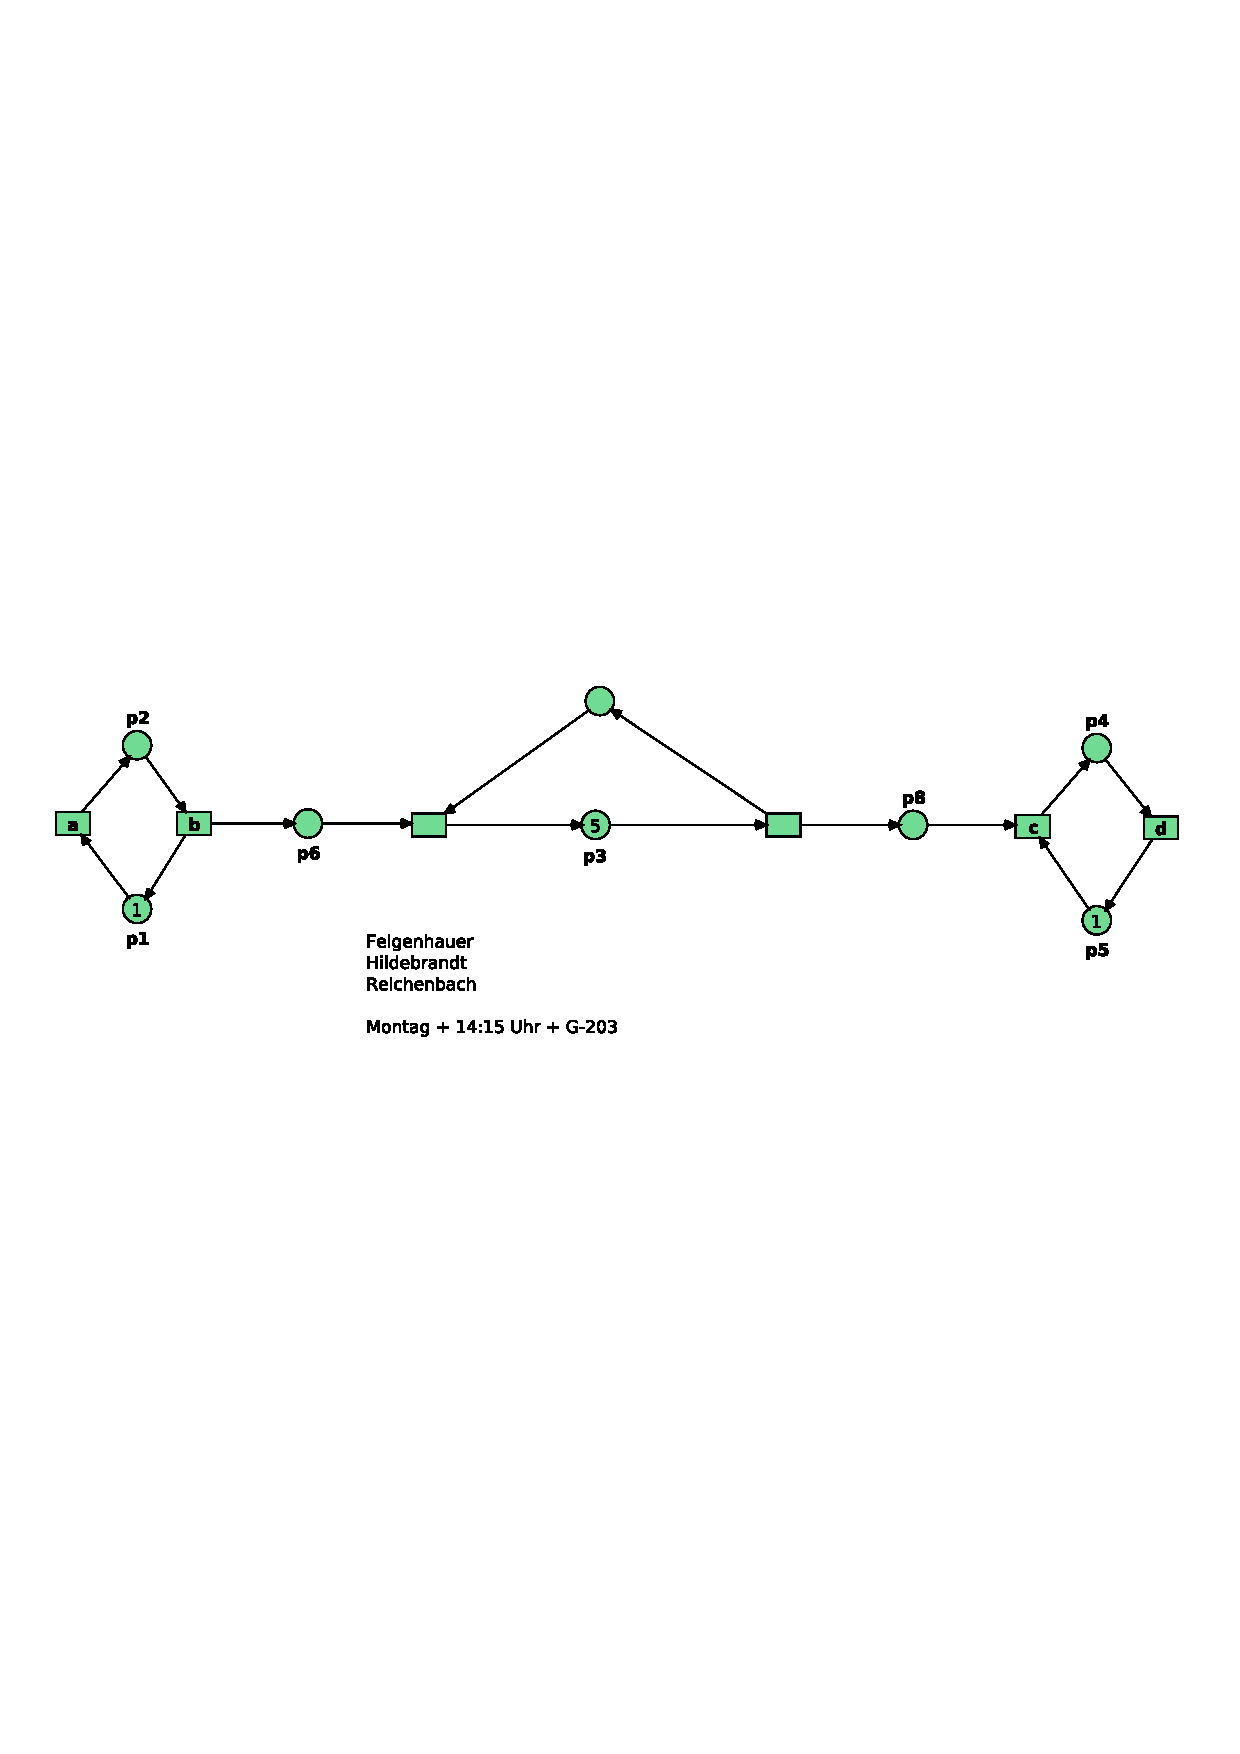
\includegraphics[scale=0.8,trim={5mm 110mm 10mm 110mm},clip]{Aufgabe_6-4/Aufgabe_6-4-7.pdf}
\includegraphics[scale=0.8,trim={0mm 225mm 10mm 0cm},clip]{Aufgabe_6-4/Aufgabe_6-4-7-sim-1.pdf}

\newpage

\includegraphics[scale=0.8,trim={0mm 225mm 10mm 0cm},clip]{Aufgabe_6-4/Aufgabe_6-4-7-sim-2.pdf}
\includegraphics[scale=0.8,trim={0mm 225mm 10mm 0cm},clip]{Aufgabe_6-4/Aufgabe_6-4-7-sim-3.pdf}
\includegraphics[scale=0.8,trim={0mm 225mm 10mm 0cm},clip]{Aufgabe_6-4/Aufgabe_6-4-7-sim-4.pdf}
\includegraphics[scale=0.8,trim={0mm 225mm 10mm 0cm},clip]{Aufgabe_6-4/Aufgabe_6-4-7-sim-5.pdf}
\end{document}